In 2013 the ATLAS 2011 data was reprocessed with improved algorithms and
calibrations. In TileCal the methods to produce Cs and laser calibration
constants were improved and required a re-computation of the TileCal noise
constants. Changing the calibration constants, according to \cref{eq:70},
changes the reconstructed energy in the cell thus affecting the jet
identification (see \cref{sec:topocluster}). A comparison between the
$\phi$--averaged RMS of electronic cell noise as a function of $\eta$ of the
cell before and after reprocessing for the high statistic run 192130 with both
channels in high gain is shown in \cref{fig:noise_avg_old_new_hghg}. There is a
general increase of the cell noise of about 0.5\% in the EBC, LBC and EBA
partitions. The LBA partition had module 22 running in \emph{emergency mode},
i.e.\ operated with $\sim$ 50~V less high voltage on the PMTs, and had the
cesium calibration constants updated. This change is likely to have lowered the
average noise in this partition.

\begin{figure}[!h]
  \centering
    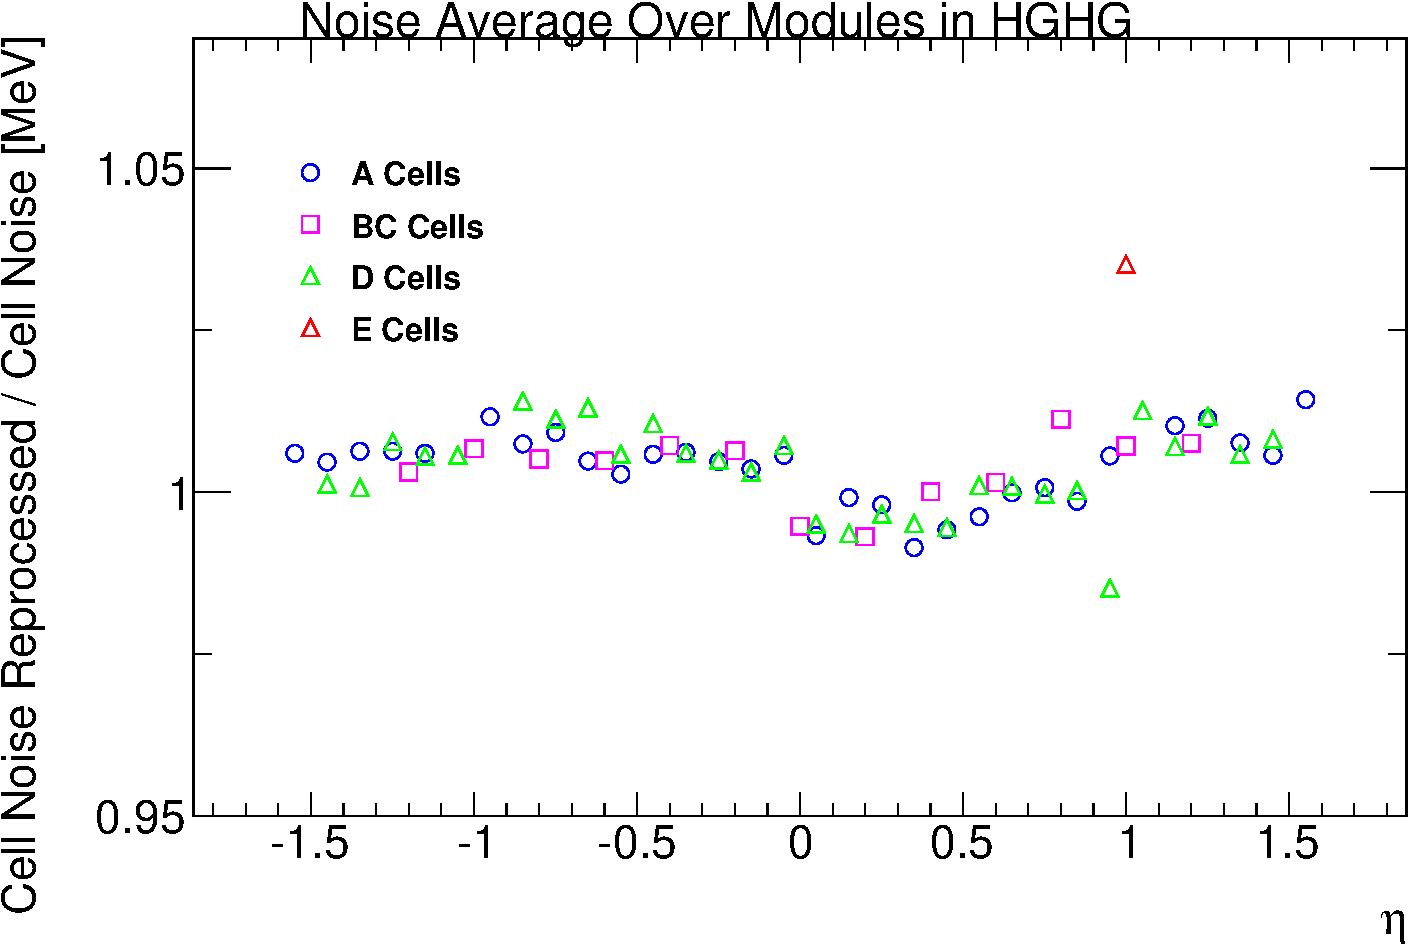
\includegraphics[width=.8\linewidth]{noise_avg_old_new_192130_hghg}
    \caption{Comparison between the $\phi$--averaged RMS of electronic cell
      noise as a function of $\eta$ of the cell before and after reprocessing
      for the high statistic 192130 run with both channels in high gain. The
      different layers are shown separately, A, BC, D and E (gap/crack). The
      transition between the long and extended barrels can be seen in the range
      $0.7 < |\eta| < 1.0$.}
    \label{fig:noise_avg_old_new_hghg}
\end{figure}

The change of the cell noise between IOVs was monitored using a special software
within the TUCS environment. A problem with the TNF has been identified in cells
which exhibits a variation in the cell noise without a corresponding variation
in other relevant quantities were present. The number of cells affected by this
problem is investigated constructing the distribution of the ratio $\sigma$ /
RMS$_\mathrm{\, eff}$ shown in \cref{fig:all_rms_eff}. The bulk of the
distribution have $\sigma$~/~RMS$_\mathrm{\, eff}$ close to one, this
corresponds to cells for which the double Gaussian noise is a good model. There
is nevertheless a big tail of cells with $\sigma$~/~RMS$_\mathrm{\, eff}$ up to
1.7, with about 5\% of the cells with $\sigma$~/~RMS$_\mathrm{\, eff}$ larger
than 1.2. After the installation of the new LVPS the contribution from a second
wider Gaussian to the electronic noise is much smaller and the effect of the TNF
is expected to be smaller as well. However the effect of the TNF with the new
power supplies remains to be checked.
\begin{figure}[!h]
  \centering
    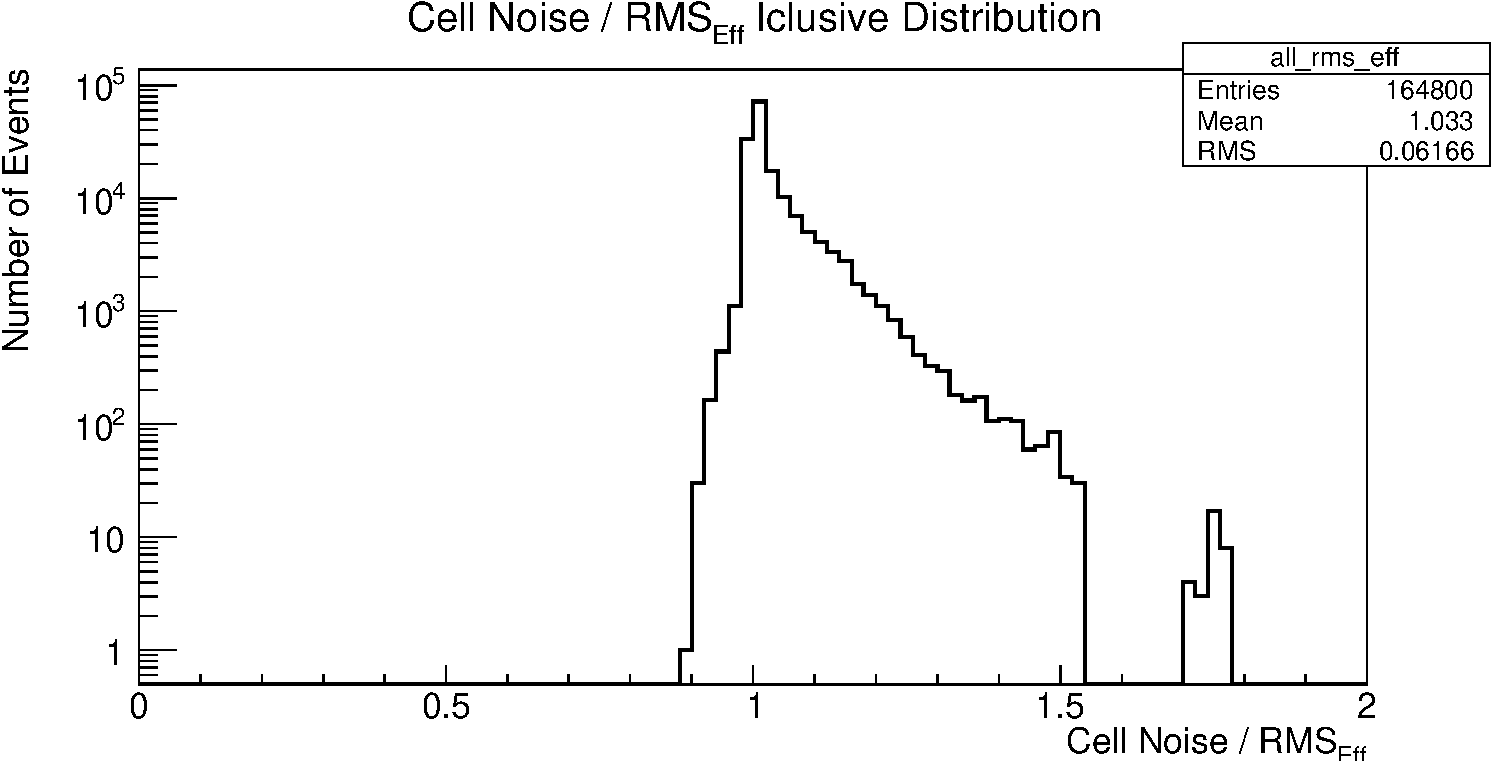
\includegraphics[width=.8\linewidth]{all_rms_eff}
    \caption{Distribution of the ratio $\sigma$ / RMS$_\mathrm{\, eff}$ where the
      $\sigma$ and RMS$_\mathrm{\, eff}$ values are taken from all IOVs
      considered for the 2011 TileCal reprocessing.}
    \label{fig:all_rms_eff}
\end{figure}
%%% Local Variables:
%%% mode: latex
%%% TeX-master: "../search_for_DM_LED_with_ATLAS"
%%% End:
